\documentclass[a4paper, 12pt, twoside]{article}
\usepackage{fancyhdr}
\usepackage{amsmath}
\usepackage{graphicx}

\pagestyle{fancy}
\fancyhf{}
\rhead{Joseph Free \\ MATH 3261 \\ Project 3}
\lhead{Application of Tridiagonal Matrix LU Decomposition}
\addtolength{\headheight}{41.7pt}
\cfoot{\thepage}

\begin{document}
\section{Problem}

In this assignment we are given an ordinary second order differential equation (Poisson's Equation in one dimension)
\begin{equation} 
\label{1}
-u''(x) = f(x)
\end{equation} 
with boundary conditions $u(0) = u(1) = 0$
and we seek to find a discrete approximate solution. We will  achieve this by rewriting $(\ref{1})$ in the approximate form
\begin{equation}
\label{2}
-v_{i+1} +2v_{i}-v_{i-1} = h^2f_i,
\end{equation}
by using the discrete analog of the second order difference quotient. Here, $x_i = ih$ and $h = 1/(n+1)$, for $i = 1,2,\dots,n$. 
 
By substituting successive values of $i$, we can express $(\ref{2})$ as the set of linear equations
\begin{equation}
\label{3}
\begin{array}{cccc}
	i = 1:& -v_0+2v_1-v_2   &=&h^2f_1\\
	i = 2:& -v_1+2v_2-v_3 &=&h^2f_2\\
	i = 3:& -v_2+2v_3-v_4 &=&h^2f_3\\
	\vdots&\vdots&\vdots&\vdots\\
	i = n:& -v_{n-1} + 2v_n - v_{n+1} &=&h^2f_n\\
\end{array}
\end{equation}
Which we can then write in matrix $Av = f$ format as
(taking $v_0 = u(0) = v_{n+1} = u(1) = 0$)
	\[
	\begin{bmatrix}
	2v_1 &-v_2  & 0   &0&0&0 &\dots &0\\
	-v_1 & 2v_2 &-v_3 & 0 & 0  & 0 &\dots &0\\
	0 &-v_2  & 2v_3 &-v_4 & 0 & 0 &\dots &0 \\
	0 & 0 & -v_3 & 2v_4 &-v_5 & 0 &\dots &0\\
	0&0&0&\ddots&\ddots&\ddots&\ddots&\vdots\\
	0&0&0&\ddots&\ddots&\ddots&\ddots&0\\
	\vdots&\vdots&\vdots&\ddots&0&-v_{n-2}&2v_{n-1}&-v_n\\
	0&0&0&\dots&0&0&-v_{n-1}&2v_n\\
	\end{bmatrix}
	\]
	\[
	=
	\begin{bmatrix}
	2 &-1  & 0   &0&0&0 &\dots &0\\
	-1 & 2 &-1 & 0 & 0  & 0 &\dots &0\\
	0 &-1  & 2 &-1 & 0 & 0 &\dots &0 \\
	0 & 0 & -1 & 2 &-1 & 0 &\dots &0\\
	0&0&0&\ddots&\ddots&\ddots&\ddots&\vdots\\
	0&0&0&\ddots&\ddots&\ddots&\ddots&0\\
	\vdots&\vdots&\vdots&\ddots&0&-1&2&-1\\
	0&0&0&\dots&0&0&-1&2\\
	\end{bmatrix}
	\begin{bmatrix}
	v_1\\
	v_2\\
	v_3\\
	\vdots\\
	\vdots\\
	\vdots\\
	v_{n-1}\\
	v_n\\
	\end{bmatrix}
	=h^2
	\begin{bmatrix}
	f_1\\
	f_2\\
	f_3\\
	\vdots\\
	\vdots\\
	\vdots\\
	f_{n-1}\\
	f_n\\
	\end{bmatrix}
	\]
Thus, we see that the problem is reduced to that of solving the tridiagonal linear system above. We will accomplish this by decomposing the coefficient matrix into upper and lower bidiagonal matrices $U$ and $L$ and solving the associated (much easier to work with) systems $Lg = f$ and $Uv=g$ for the n dimensional vector $v$.

Note that the vector $v$ is exactly that
which has components $v_i$ satisfying the ith equation of (\ref{3}). That is, $v_i$ is an approximation of the value 
$u(x_i)$. Hence, the vector $v$ is a collection of n points approximating the function $u(x)$.


For this assignment we will be assuming that $f(x) = 100e^{-10x}$. With this choice of $f$, $(\ref{1})$ has closed solution $u(x) = 1-(1-e^{-10})x-e^{-10x}$, which we will be comparing our approximations to for various choices of n. 

To verify that $u(x)$ as given is a solution of $(\ref{1})$, refer to the following calculation.
$$
\begin{array}{ccc}
	-u''(x)& = & -[1-(1-e^{-10})x-e^{-10x}]''\\
	&=&-[(1-e^{-10}) + 10e^{-10x} ]'\\
	&=&-(-100e^{-10x})\\
	&=& 100e^{-10x}\\
	&=& f(x)\\
\end{array}
$$

\newpage
\section{Source Code}

$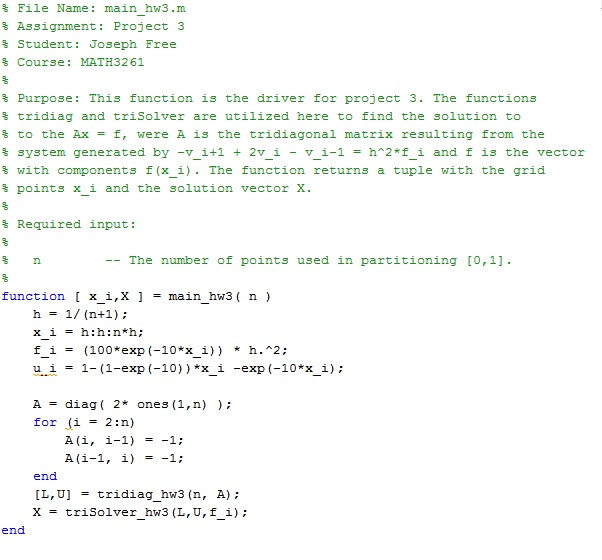
\includegraphics{code_main}$
\newpage
$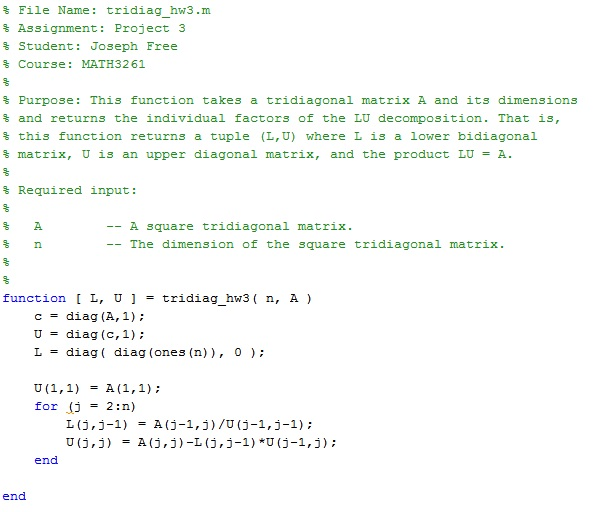
\includegraphics{code_tridi}$
\newpage
$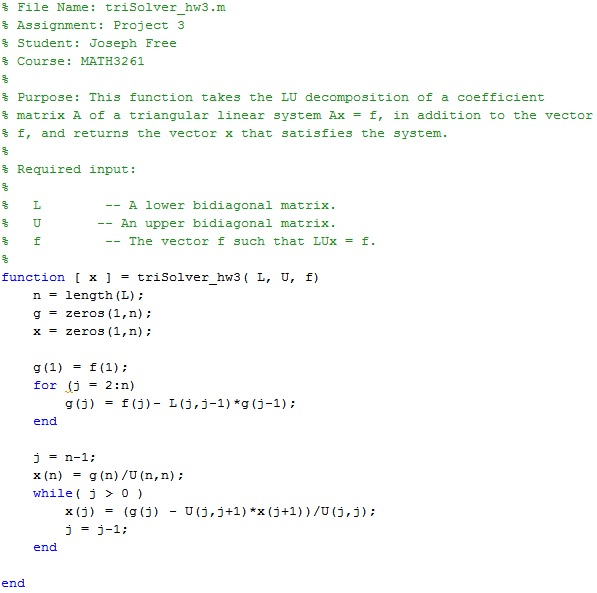
\includegraphics{code_triSolver}$
\newpage
\section{Results}

Using the code from section two, five sets of approximations were made for n = 10, 25, 40, 50, and 1000. For each approximate solution, plots were made against the exact solution $u(x) = 1-(1-e^{-10})x-e^{-10x}$ and relative error
E calculated in order to determine accuracy.

As was to be expected, the approximation using n = 10 points was hardly accurate. However, for larger values of n, $v$ tended to approach $u(x_i)$ very rapidly. In fact with just 25 points, 
$v$ does an admirable job of approximating the solution of (\ref{1}).\\
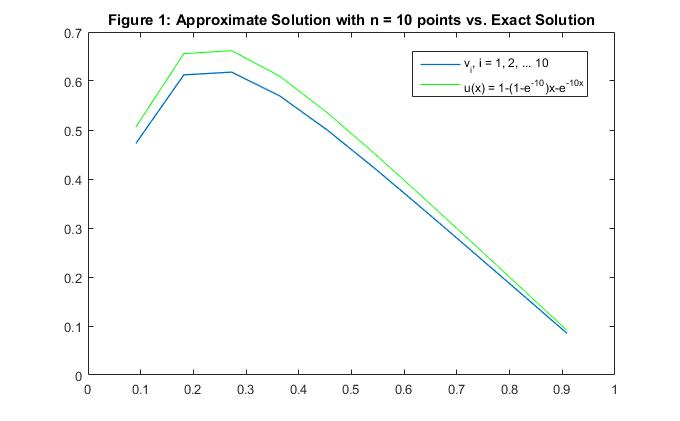
\includegraphics[scale=.5]{fig1}\\
Relative error, $E = -1.17969$\\
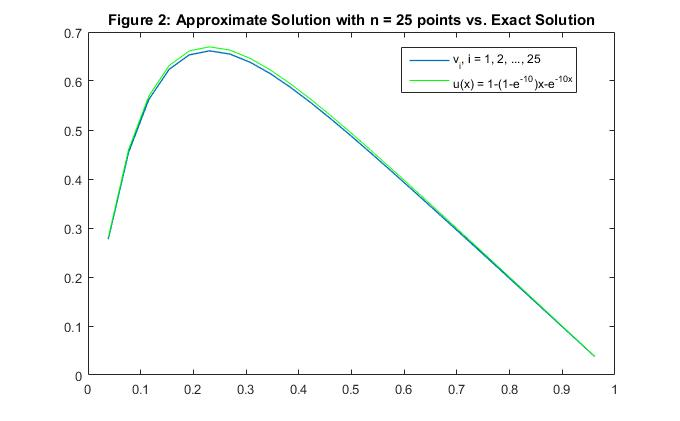
\includegraphics[scale=.5]{fig2}\\
Relative error, $E = -1.91233$\\
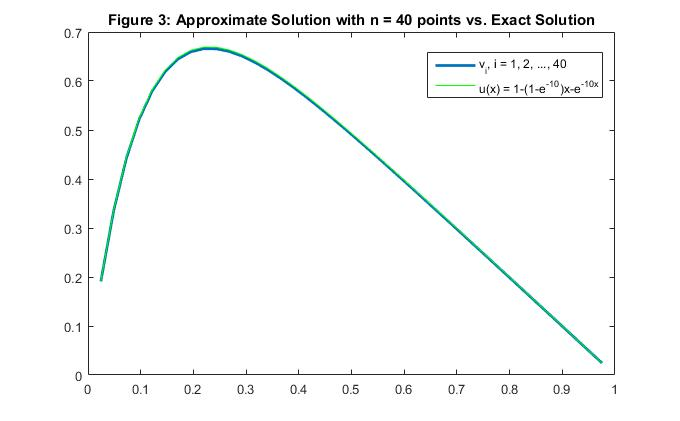
\includegraphics[scale=.5]{fig3}\\
Relative error, $E =-2.30603$\\
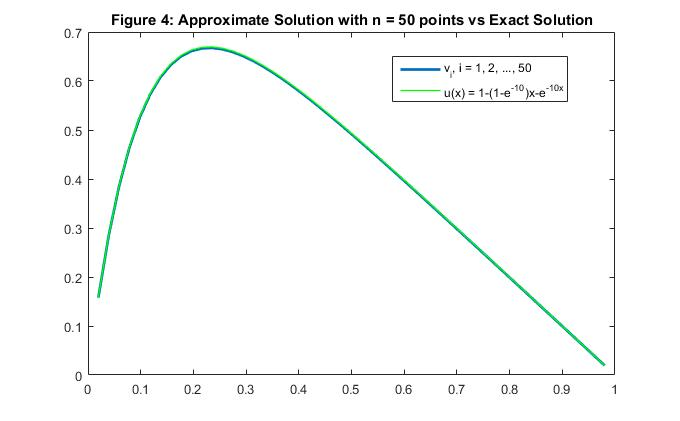
\includegraphics[scale=.5]{fig4}\\
Relative error, $E =-2.49515$\\
\newpage
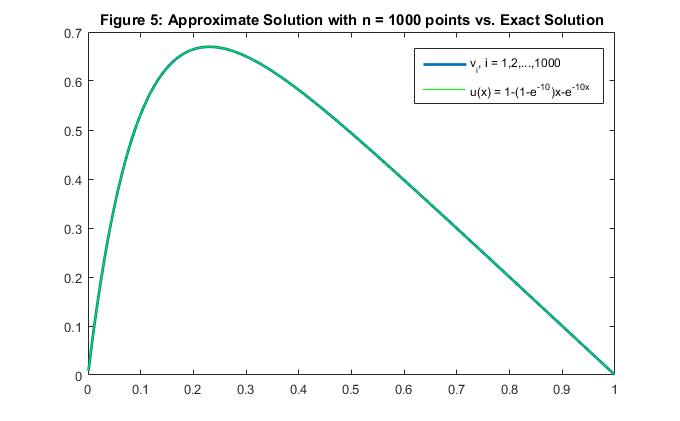
\includegraphics[scale=.5]{fig5}\\
Relative error, $E =-5.08005$\\

\end{document}
